\documentclass[12pt,notitlepage,nofootinbib]{revtex4}
\usepackage{graphicx}
\usepackage{bm}
\usepackage{rotating}
\def\baselinestretch{1.2}
\usepackage{dcolumn}
\usepackage{times}
\usepackage{color}
\usepackage{amsmath,amssymb,amsfonts} 
\usepackage{extarrows}
\usepackage{listings}
\usepackage{url}
\setlength{\mathindent}{0pt}

\begin{document}

\title{StochSS Hands-on Tutorial Series: 3 - StochOptim: Parameter Estimation with StochSS}

\author{StochSS Development Team}
\affiliation{Department of Computer Science - University of California, Santa Barbara}

\date{\today}

\maketitle

\section{\label{sec:pre}Prerequisites}
\begin{itemize}
\item StochSS 1.4 (or later) installed on your computer (please follow download and installation instructions at \url{www.stochss.org}). 
\item A basic understanding of well-mixed discrete stochastic simulations and models based on ordinary differential equations \cite{dan,sundials}.
\item A basic knowledge of the MCEM$^2$ method \cite{bernie,dan,caffo}. 
\item  A basic familiarity with the StochSS GUI (please consult the \textit{Basic Introduction to StochSS} tutorial).
\item The following login screen appears in your browser; please log in.
\end{itemize}

\begin{figure}[!htb]
\centering
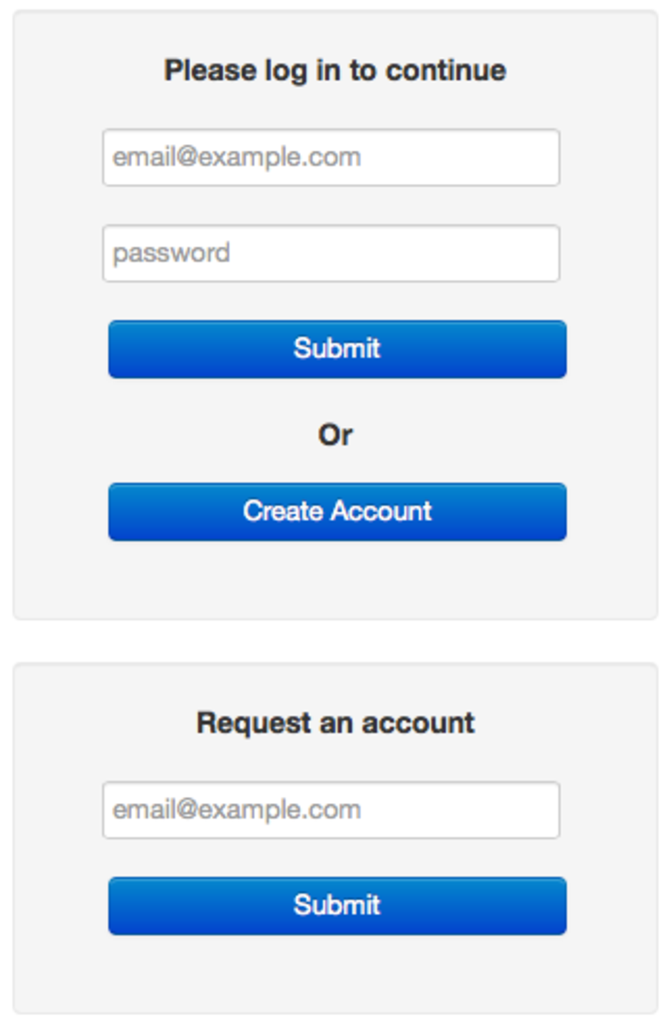
\includegraphics[scale=0.6]{user-login.pdf}
\end{figure}

\section{StochOptim: Parameter Estimation for Stochastic Biochemical Systems}
StochSS implements parameter estimation for stochastic biochemical systems (StochOptim) via the Monte Carlo expectation-maximization with Modified Cross-Entropy method (MCEM$^2$) \cite{bernie}.
MCEM$^2$ computes maximum likelihood parameter estimates (MLEs) and associated uncertainties in three consecutive phases: cross-entropy, Monte Carlo expectation-maximization (MCEM), and uncertainty quantification \cite{bernie}.

\subsection{An Instructive Example}
We consider the Birth-Death model that can be imported from the StochSS Public Library (see the \textit{Introduction to StochSS} tutorial for instructions on how to import models in StochSS).
After the model has been imported:
\begin{itemize}
\item \textbf{Select} \textcolor{blue}{Parameter estimation} from the menu on the left of the screen.
\item \textbf{Click} on the \textcolor{blue}{Next} button (make sure that the right model is selected). This will open the Simulation page.
\item On the Simulation page, \textbf{select} only parameter k1. In this example the default value of k2 is already optimized. This is done to make the convergence process faster. Upload the data files that will be used for the parameter estimation.
\item Example files (StochOptim input data) for the initial conditions and the trajectories are provided in the \textit{examples} folder (included in your StochSS package) and are named \textit{birthDeathInitial.txt} and \textit{birthDeathTrajectories.txt}, respectively.
\item Now we are ready to start the parameter estimation routine clicking on the \textcolor{blue}{Run Locally} button at the bottom of the page. 
\item \textbf{Select} \textcolor{blue}{Job Status} from the menu on the left of the screen to monitor the status of your running calculation.
\textbf{Click} on  \textcolor{blue}{View Progress} to access the Job Summary page and view more details about your calculation status. \textit{Note:} parameter estimation calculations using MCEM$^2$ are typically time consuming, intensive calculations. For this simple example, the parameter estimation process took about $9-10$ minutes on a Macbook Pro (Intel Core i7 - 2011). By selecting both k1 and k2 parameters the parameter estimation process took about $90$ minutes on the same machine.

\item When the job has successfully ended, you can generate a new model using the final estimates of the MCEM$^2$ calculation as follows: scroll to the bottom of the Job Summary page and \textbf{click} on the \textcolor{blue}{Create Model from Current Estimates} button. 
\item If the job doesn't complete in a reasonable amount of time the job can be stopped manually on the \textcolor{blue}{Job Status} page and the parameters can be extracted using the \textcolor{blue}{Create Model from Current Estimates} button.
\end{itemize}

\subsection{StochOptim file format}
The StochOptim input data format consists of two, tab-separated text-based input files.
The first file represents the initial conditions of the system, and the second file represents trajectories of it.
Each file has three base columns. \textit{Time}, \textit{Rep}, and \textit{Weight}. Additional columns are added for every species in the model that parameter estimation is to be run on. The \textit{Time} column contains the time values of the various trajectories (and should be set to zero for the initial conditions file). The \textit{Rep} column is used to include multiple trajectories in one file for fitting. Basically each trajectory should have a different \textit{Rep} number. An example of this can be seen by comparing the files \textit{birthDeathTrajectories.txt} and \textit{birthDeathTrajectoriesMulti.txt} in the \textit{examples} folder included in the StochSS package. The \textit{Weight} column is currently unused and should be set to $1$. The rest of the columns should be named after the species (case-sensitive) in the model the data will be fit against, and the columns themselves should contain integers representing the population counts at the various time points.

\newpage

\begin{thebibliography}{9}
  
  \bibitem{dan}
  D.T. Gillespie.
  \textit{Exact stochastic simulation of coupled chemical reactions}.
  J. Phys. Chem., 81(25), 2340-2361 (1977)
  
  \bibitem{sundials}
  A. C. Hindmarsh et al.,
  \textit{SUNDIALS: Suite of nonlinear and differential/algebraic equation solvers}.
  ACM Trans. Math. Softw., 31(3), 363-396 (2005)
  
  \bibitem{bernie}
  B.J. Daigle et al.
  \textit{Accelerated maximum likelihood parameter estimation for stochastic biochemical systems}.
  BMC Bioinformatics, 13, 68 (2012)
  
  \bibitem{caffo}
  B.S. Caffo et al.
  \textit{Ascent-based Monte Carlo expectation-maximization}. 
  J. Royal Statistical Society Series B, 67(2), 235-251 (2005)
  
\end{thebibliography}

\end{document}
